
\section{Assets Information Model}
\label{sec:Assets Information Model}

The MTConnect Standard supports a simple distributed storage mechanism that allows applications and equipment to share and exchange complex information models in a similar way to a distributed data store.  The \gls{Assets Information Model} associates each electronic \block{MTConnectAssets} document with a unique identifier and allows for some predefined mechanisms to find, create, request, updated, and delete these electronic documents in a way that provides for consistency across multiple pieces of equipment.

The protocol provides a limited mechanism of accessing \glspl{MTConnect Asset} using the following properties: \property{assetId}, \gls{Asset} type (element name of \gls{Asset} root), and the piece of equipment associated with the \gls{Asset}.  These access strategies will provide the following services and answer the following questions: What \glspl{Asset} are from a particular piece of equipment?  What are the \glspl{Asset} of a particular type? What \glspl{Asset} is stored for a given \property{assetId}?

Although these mechanisms are provided, an \gls{agent} should not be considered a data store or a system of reference.  The \gls{agent} is providing an ephemeral storage capability that will temporarily manage the data for applications wishing to communicate and manage data as need-ed by the various processes.  An application cannot rely on an \gls{agent} for long term persistence or durability since the \gls{agent} is only required to temporarily store the \gls{Asset} data and may require an-other system to provide the source data upon initialization.  An \gls{agent} is always providing the best-known equipment centric view of the data given the limitations of that piece of equipment.

The following sections provide the semantic information for the \block{Asset} model.

\input model-sections/Assets.tex

\section{CuttingTool Asset Information Model}
\label{sec:CuttingTool Asset Information Model}

MTConnect Standard will adopt the ISO 13399 structure when formulating the vocabulary for Cutting Tool geometries and structure to be represented in the \block{CuttingToolArchetype}. The nominal values provided in the \block{CuttingToolLifeCycle} section are only concerned with two aspects of the Cutting Tool; the Cutting Tool and the Cutting Item. The Tool Item, Adaptive Item, and Assembly Item will only be covered in the \block{CuttingToolDefinition} section of this document since this section contains the full ISO 13399 information about a Cutting Tool.

\begin{figure}[ht]
  \centering
    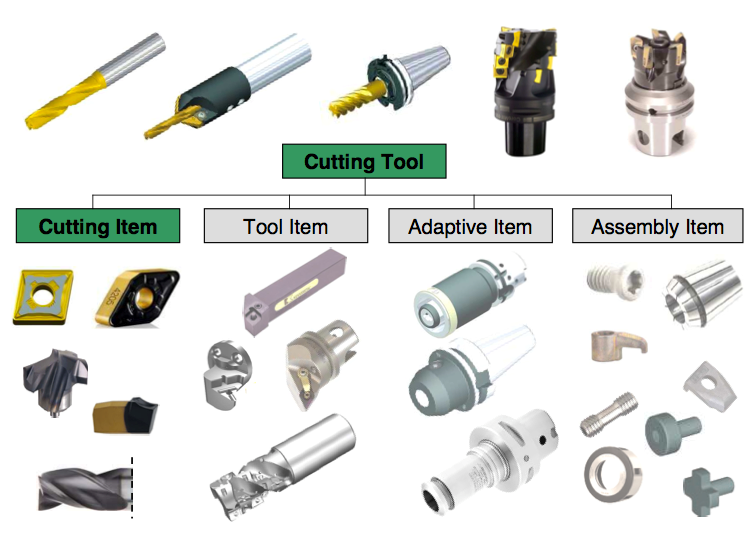
\includegraphics[width=1.0\textwidth]{figures/Cutting Tool Parts.png}
  \caption{Cutting Tool Parts Diagram}
  \label{fig:Cutting Tool Parts Diagram}
\end{figure}

\FloatBarrier


The \fig{Cutting Tool Parts Diagram} illustrates the parts of a Cutting Tool. The Cutting Tool is the aggregate of all the components and the Cutting Item is the part of the tool that removes the material from the workpiece. These are the primary focus of the MTConnect Standard.

\begin{figure}[ht]
  \centering
    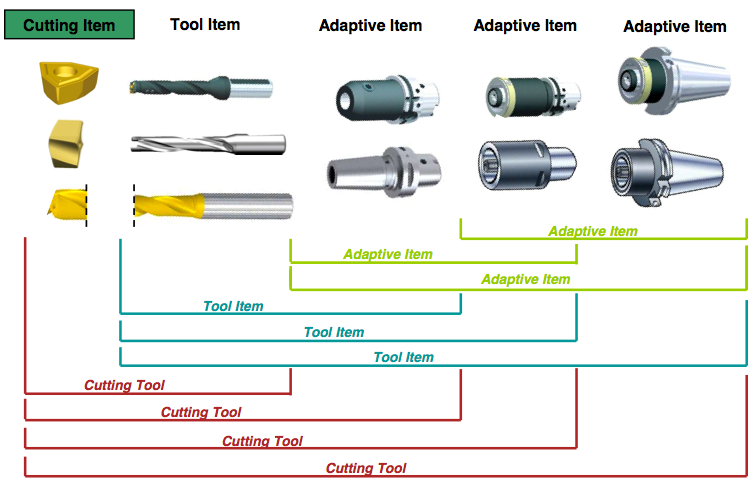
\includegraphics[width=1.0\textwidth]{figures/Cutting Tool Composition.png}
  \caption{Cutting Tool Composition Diagram}
  \label{fig:Cutting Tool Composition Diagram}
\end{figure}

\FloatBarrier


\fig{Cutting Tool Composition Diagram} provides another view of the composition of a Cutting Tool. The Adaptive Items and Tool Items will be used for measurements, but will not be modeled as separate entities. When we are referencing the Cutting Tool we are referring to the entirety of the assembly and when we provide data regarding the Cutting Item we are referencing each individual item as illustrated on the left of the previous diagram.

!Cutting Tool, Tool Item, Cutting Item.png!

!Cutting Tool, Tool Item, Cutting Item 2.png!

{{fig(Cutting Tool, Tool Item, Cutting Item Diagram)}} and {{fig(Cutting Tool, Tool Item, Cutting Item 2 Diagram)}} further illustrates the components of the Cutting Tool. As we compose the Tool Item, Cutting Item, Adaptive Item, we get a Cutting Tool. The Tool Item, Adaptive Item, and Assembly Item will only be in the \block{CuttingToolDefinition} section that will contain the full ISO 13399 information. These figures also use the ISO 13399 codes for each of the measurements. These codes will be translated into the MTConnect Standard vocabulary as illustrated below. The measurements will have a maximum, minimum, and nominal value representing the tolerance of allowable values for this dimension.

The MTConnect Standard will not define the entire geometry of the Cutting Tool, but will provide the information necessary to use the tool in the manufacturing process. Additional information can be added to the definition of the Cutting Tool by means of schema extensions.

Additional diagrams will reference these dimensions by their codes that will be defined in the measurement tables. The codes are consistent with the codes used in ISO 13399 and have been standardized. MTConnect Standard will use the full text name for clarity in the \glspl{Response Document}.



\input model-sections/CuttingTool.tex

\input model-sections/CuttingToolLifeCycle.tex

\input model-sections/CuttingItem.tex

\input model-sections/CuttingToolMeasurementTypes.tex

\input model-sections/CuttingItemMeasurementTypes.tex

\section{Files Asset Information Model}
\label{sec:Files Asset Information Model}

Manufacturing processes require various documents, programs, setup sheets, and digital media available at the device for a given process. The \block{File} and \block{FileArchetype} \block{Asset}s provide a mechanism to communicate specific "Files" that are relevant to a process where the media is located on a server and represented by a Universal Resource Locator (URL).

The \block{FileArchetype} contains metadata common to all \block{File} \block{Asset}s for a certain purpose. The \block{File} \block{Asset} references the file specific to a given device or set of devices. The \block{File} \block{Asset} does not hold the contents of the file, it contains a reference to the location (URL) used to access the information. The metadata associated with the \block{File} provides semantic information about the representation (mime-type) and the application associated with the \block{File}. The application of the file is an extensible controlled vocabulary with common manufacturing uses provided.

\input model-sections/Files.tex

\section{RawMaterial Asset Information Model}
\label{sec:RawMaterial Asset Information Model}

Raw material represents the source of material for immediate use and sources of material that may or may not be used during the manufacturing process.

The \block{RawMaterial} \block{Asset} holds the references to the content stored in the actual \block{RawMaterial} container or derived about the \block{RawMaterial} by the system during operation.

\input model-sections/RawMaterial.tex

\section{QIF Asset Information Model}
\label{sec:QIF Asset Information Model}

The Quality Information Framework (QIF) is an American National Standards Institute (ANSI) accredited standard developed by the Digital Metrology Standards Consortium (DMCS) standards development organization and an A-liaison to the International Standards Organization (ISO) Technical Committee (TC) 184. QIF addresses the needs of the metrology community to have a semantic information model for the exchange of metrology data throughout the verification lifecycle from product design to execution, analysis, and reporting.

The MTConnect QIF Asset Information Model provides a wrapper around the QIF Information model in its native XML representation utilizing the QIF XML Schema Definition Language (XSDL) references in the wrapper to validate the document. The MTConnect standard does not alter or extend the QIF standard and regards the QIF standard as a passthrough.

Information about the QIF standards is at the following location: https://qifstandards.org

\input model-sections/QIF.tex
